
% % % % % % %  THE TEMPLATE TILL THE TITLE CAN BE USED AS IT IS%%%%%%%%%%%%%%%%%%%%%%%
% % % you are going to need revtex4-1 on your machine..........
\documentclass[prl,12pt,citeautoscript,reprint]{revtex4-1}
%\documentclass[preprint,12pt]{revtex4}
\usepackage{graphicx}
\usepackage{verbatim}
\usepackage{epsfig}
\usepackage{amsmath}
\usepackage{graphicx}% Include figure files
\usepackage{dcolumn}% Align table columns on decimal point
\usepackage{bm}% bold math
\usepackage{amssymb}
\usepackage{amsmath}
\usepackage{epsf}
\usepackage{subfigure}
\usepackage{epstopdf}
\usepackage{color}
\usepackage{subeqnarray}
\usepackage{mathrsfs}
\usepackage{float}
\usepackage[colorlinks=true, pdfstartview=FitV, linkcolor=red, citecolor=blue, urlcolor=blue]{hyperref}
\newcommand{\be}{\begin{equation}}%% begin equation
\newcommand{\ee}{\end{equation}} %% end equation
\newcommand{\ben}{\begin{eqnarray}} %% begin equation array
\newcommand{\een}{\end{eqnarray}} %%% end equation array
\begin{document}
\title{Wolf Sheep Predation: Cellular Automata Model }
\author{Akshay Miterani (ID:201401443)}
\email{201401443@daiict.ac.in}
\author{Mihir Limbachia (ID:201401456)}
\email{201401456@daiict.ac.in}



\affiliation{CS-302 Modeling and Simulation course, DA-IICT}


% % % % % Abstract provides an overview of what has been done in the article
\begin{abstract}
We consider a cellular automata model of predator prey model with agents sheep and wolf in the cellular matrix.This model consists of sheep consuming grass , wolf consuming sheep, sheep and wolf reproducing and dying when starved. Depending on the parameters selected the model shows fascinating behaviour.
\end{abstract}
\maketitle
\section{Introduction}
Predator prey model has always fascinated scientists and researchers. The Vito Volterra\cite{Volterra1931} and Alfred Lotka 's\cite{Lotka1920} system dynamic models considers the species interaction but does not take into account individual variations.Certain cellular automata models have been developed to consider different aspects of natural life, including motion, birth and death processes, evolution and extinction.However here we consider the model developed by He, Mingfeng, Hongbo Ruan, and Changliang Yu.\cite{He2003} and use simplified rules from the model given in the book Intro to Computational Science: Modeling and Simulation Angela \cite{Shifet} to model a sequential version of model.  
\section{Model}
% %  DISCUSS THE MODEL AND ANY OTHER DETAILS

First of all lets discuss the assumptions and implementation of various grids in our model.

Grass Grid Assumptions and Implementation:

\begin{itemize}
\item In this system we consider a grass grid signifying the presence/absence of grass in a matrix.Also since we have a condition in the rule that says the grass regrowth time is 4 time steps. We set the presence of grass in the grid as 4.We regard 0 as temporarily barren which will in 4 time steps be with grass again. 
\item We do initialization considering the probability of presence of grass at that place.
\item We also increase the temporarily barren cell's value by 1 every time step to make it regrown with grass in 4 time steps. 
\end{itemize}

The reason for implementing separate grass grid and animal grid is to accommodate the situation where animal ends up on grass.
\\
 Animal Grid Assumptions:
\begin{itemize}
\item We assume that there is no collision between the animals.
\end{itemize}
For interaction between the agents we consider Moore neighborhood and extend the matrix with constant boundary conditions set to BORDER value indicating no interaction. 

Morover the animal's attributes ration and age are recorded in different matrix for convenience.
We set a fixed amount of ration that an animal can have and the animals ration varies between 1 and that fixed amount.
Modeling Basic functions of animals:

\begin{enumerate}

 \item Movement
 \begin{itemize}	 
 \item allocating sheep a location in neighborhood preferably with grass 
 \item allocating wolf a location in neighborhood preferably with sheep    
 \end{itemize}
 
  \item Consumption
  \begin{itemize}
  	\item If a sheep has ration less than the maximum it can have it consumes grass at its location or moves to a neighboring location with grass and consumes it. The sheep's ration increases by a certain fixed amount which is termed as sheep energy gain.
  	\item If a wolf has ration less than the maximum it tries to hunt and find  a sheep in neighborhood if present else just moves to a random empty cell. The wolf's ration increases by a certain fixed amount which is termed as wolf energy gain.
  \end{itemize}
  \item Reproduction
  \begin{itemize}
  \item Each animal has a certain reproduction age and a reproduction ration assigned to it beyond which it can reproduce.
  \item When an animal reproduces its ration reduces by half and that is assigned to the new born. The gender of the new born is randomly assigned with equal probability.    
  \end{itemize}
  \item Aging and Death
  \begin{itemize}
  \item The age of each animal is increased by one unit each time step
  \item The ration of each animal is reduced by one unit each time step. The animal who has no ration assigned to it dies by removal from  the grid cell.	  
\end{itemize}  	  
\end{enumerate}
 Thus the basic functions of animal life are successfully implemented in this model with individual variations.
\\ 
 The parameters that need to be set for this model are:
  \begin{itemize}
  \item grid size
  \item Number of wolves and sheep
  \item Wolf and sheep energy gain
  \item Wolf and sheep max ration
  \item Wolf and sheep reproduction age and ration 
  \end{itemize}
These parameters need to be tuned to get situations where: 
\begin{enumerate}
\item both the species go extinct or the wolfs become extinct
\item Only the wolfs become extinct. 
\end{enumerate}

% % %  For multiple equations you can use equation array

\section{Results}
In here we present the results of our numerical and analytical analysis on the model of the previous section. 
\subsection{Situation where only wolves  become extinct}
The cases where the wolf energy gain is too high that they keep on hunting sheep and then reproducing that so few remain that they are too difficult to hunt in few time steps they have based on their ration.
\\Example:\\
The parameters for the model are:\newline
$ grid size = 30x30 $\\
$sheep energy gain = 4$\\
$wolf energy gain = 25$\\
$sheep reproduction age=8$\\
$wolf reproduction age=8$\\
$reproduction sheep ration=4$\\
$reproduction sheep ration=8$\\
$max sheep ration=2*(sheep energy gain)$\\
$max wolf ration=3*(wolf sheep energy gain);$\\

\%begin{comment} 
The model with these parameter produces following plots
\begin{itemize}
\item Population plot
\begin{figure}[H]
\centering
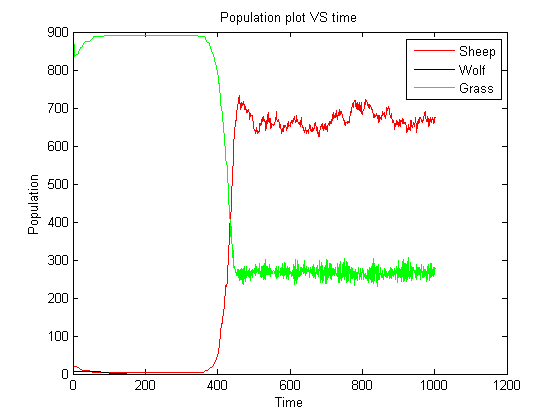
\includegraphics[width = 0.8\columnwidth]{a} 

\caption{The wolf, sheep and grass populations along 1000 time steps}\label{Fig:Population vs time}
\end{figure}
\item Cellular Matrix 
\begin{figure}[H]
\centering
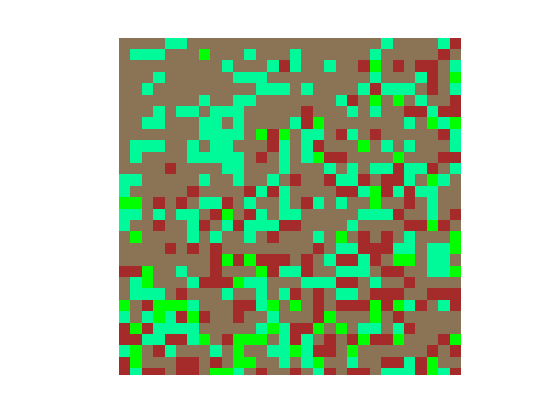
\includegraphics[width =0.8\columnwidth]{b} 
 
\caption{Cellular matrix at 1000 time step}\label{Fig:Cellular matrix at 1000 time step}
\end{figure}

\item Average Population 
\begin{figure}[H]
\centering
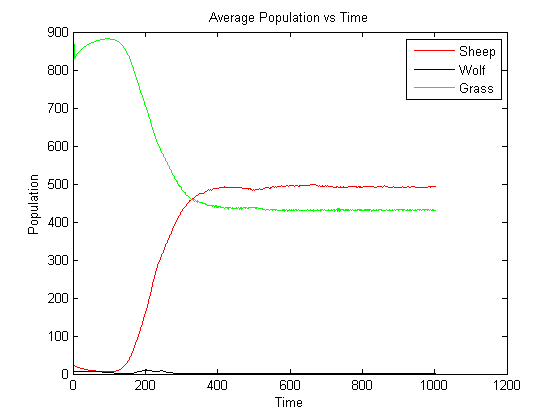
\includegraphics[width = 0.8\columnwidth]{c} 
 
\caption{Average Population over 100 iterations and 1000 time steps}\label{Fig:Cellular matrix at 1000 time step}
\end{figure}

\end{itemize}
%\end{comment}
 
\section{Situation where both species becomes extinct}
The cases where no of sheep is too large for the grid makes it easy for wolves to hunt them and that reduces the sheep population.Also since there are too many sheep the time it takes to regrow the grass is too large for the sheep to persist and the wolves because of shortage of sheep become extinct.This situation replicates the shortage of resources situation in real world.\newline
Example : \newline
The parameters for the model are:\newline
$ grid size = 10x10 $\\
$no of sheep=50$\\
$no of wolf=4$\\
$sheep energy gain = 4$\\
$wolf energy gain = 7$\\
$sheep reproduction age=8$\\
$wolf reproduction age=8$\\
$reproduction sheep ration=4$\\
$reproduction sheep ration=8$\\
$max sheep ration=2*(sheep energy gain)$\\
$max wolf ration=2*(wolf sheep energy gain);$\\
%\begin{comment} 
The model with these parameters produces following plots
\begin{itemize}
\item Population plot
\begin{figure}[H]
\centering
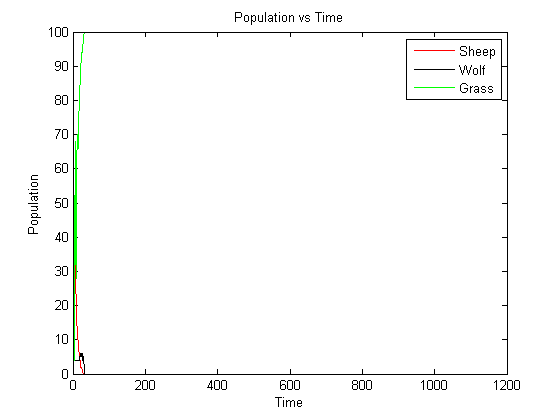
\includegraphics[width = 0.8\columnwidth]{2a} 

\caption{The wolf, sheep and grass populations along 1000 time steps}\label{Fig:Population vs time}
\end{figure}
\item Cellular Matrix 
\begin{figure}[H]
\centering

\includegraphics[width =0.8\columnwidth]{2b} 
 
\caption{Cellular matrix at 1000 time step}\label{Fig:Cellular matrix at 1000 time step}
\end{figure}

\item Average Population 
\begin{figure}[H]
\centering
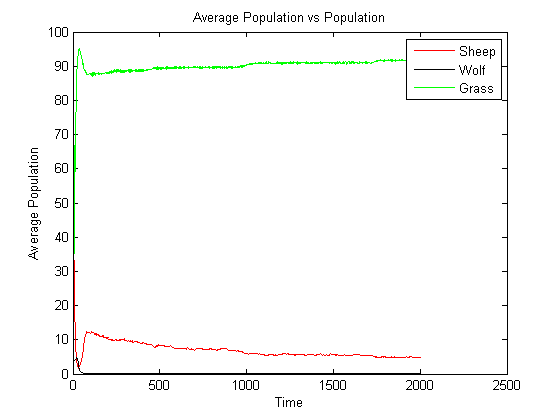
\includegraphics[width = 0.8\columnwidth]{2c} 
 
\caption{Average Population over 100 iterations and 2000 time steps}\label{Fig:Cellular matrix at 2000 time step}
\end{figure}

\end{itemize}
%\end{comment}

\section{Situation where both species becomes coexist}
In Lotka and Volterra's model, these are cases where the no of sheep is such that it can evolve to population that can exist by satisfying its ration enough using the grass population at every time step and then almost stabilizing with certain periodic motion along the population axis w.r.t time axis and the wolf population is such that it can evolve to population that can be exist by satisfying its ration enough with the sheep population and then almost stabilizing with certain periodic variation and coexisting with the sheep population lead to both species coexisting. But this model has certain changes the reasons for which are explained in analysis of model.

Example : \newline
The parameters for the model are:\newline
$ grid size = 100x100 $\\
$no of sheep=1000$\\
$no of wolf=100$\\
$sheep energy gain = 4$\\
$wolf energy gain = 16$\\
$sheep reproduction age=8$\\
$wolf reproduction age=8$\\
$reproduction sheep ration=4$\\
$reproduction sheep ration=8$\\
$max sheep ration=2*(sheep energy gain)$\\
$max wolf ration=2*(wolf sheep energy gain);$\\
 
The model with these parameters produces following plots:
\begin{itemize}
\item Population plot
\begin{figure}[H]
\centering
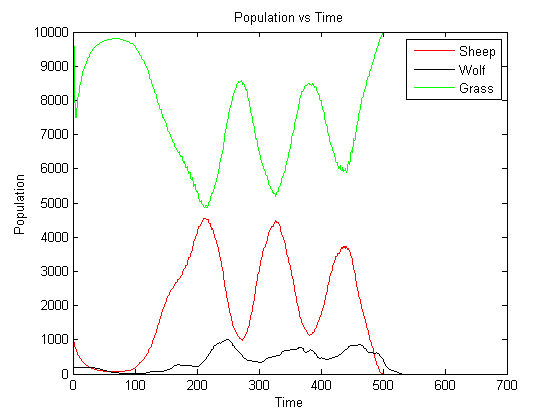
\includegraphics[width = 0.8\columnwidth]{3a} 

\caption{The wolf, sheep and grass populations along 600 time steps}\label{Fig:Population vs time}
\end{figure}
\item Cellular Matrix 
\begin{figure}[H]
\centering

\includegraphics[width =0.8\columnwidth]{3b} 
 
\caption{Cellular matrix at 600 time step}\label{Fig:Cellular matrix at 600 time step}
\end{figure}

\item Average Population 
\begin{figure}[H]
\centering
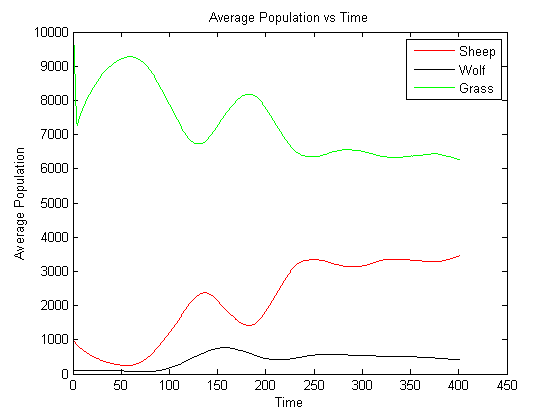
\includegraphics[width = 0.8\columnwidth]{3c} 
 
\caption{Average Population over 100 iterations and 400 time steps}\label{Fig:Cellular matrix at 600 time step}
\end{figure}

\end{itemize}
\subsection{Analysis of Model :}

However since this is a random model taking into consideration individual variability of the agents. This behaviour can only continue for certain time interval.The Lotka and Volterra's system dynamic model considered all the species as one entity behaving in same way making it come to a stabilizing situation than replicating the situation over and over in a periodic time interval. The situation changes in a cellular automata's model; Situation arises where subsequent stable configuration (The population of prey and predator ) changes. And eventually predator becomes extinct depending on the grid size.This is caused mainly by the predator individuality assimilating at some point and leading to reproduction on a drastic scale leading to eventual drastic hunting of prey causing either extinction of prey and hence predator itself or the prey surviving but not enough for the predator to survive causing predator extinction.This model thus lacks that collective co-ordination of species in terms of reproduction where only portion of species reproduces even though it has opportunity to reproduce.This kind of behaviour leads to decrease in probability of survival of one or both the species.This fact is observed by trying the same model parameters with different time intervals and concluding that even though the grid is large enough to satisfy the prey population and predator population the individuality and lack of collaboration of agents leads to either eventual extinction of both species or the predator species with later one more likely in cases of periodic variations occurring before the extinction of one or both the species.

\subsection{Evaluating Pros and Cons}
\begin{itemize}
\item Pros of Model:
\begin{enumerate}
\item This model takes into account that not all agents of each species interact with every agent of other species by implementing in the form of neighborhoods in cellular matrix.
\item This model takes in account the situations involved in death of agents in a better way using starvation
(for both prey and predator) and being hunted(prey) as the main factor implemented using neighborhood in the cellular matrix.
\end{enumerate}

\item Cons of Model:
\begin{enumerate}
\item The model does not take into account the fact that only certain portion of the species reproduces at a certain time step leading the predator to not coexist for long with the prey.
\item This model does not take age into consideration in terms of the death and reproduction.
\item This model does not take into consideration the element of chance in terms of consumption of prey by the predator which too leads to both species becoming extinct in cases where the Lotka and Voterra model predicts coexisting behaviour.
\end{enumerate}
\end{itemize}
\section{Conclusion}
In conclusion we have implemented predator prey model on a 2D cellular automaton. Our results suggest that the model correctly represents the animal behaviour in cases of unsuitable population numbers,  improper energy gain ratios, improper grid size leading to extinction of both or only predator species as per expectation.

However in terms of situations where coexisting behaviour in terms of oscillating populations is expected, the model does tend to vary leading to extinction of prey and predator or only predator or prey taking over completely the grid and predator population remaining constant at some non-zero population unable to reproduce.This model as discussed in cons of model does not take age into consideration in term of death which leads to some irregular behaviour which is not expected.The model needs improvement in terms of con points discussed in previous section.

The results vary w.r.t to reference\cite{He2003} because of use of simplified rules and non-parallel implementation of their model

\begin{thebibliography}{}
\bibitem {Wilensky1997}Wilensky, U. (1997). NetLogo Wolf Sheep Predation model. 
Center for Connected Learning and Computer-Based Modeling, Northwestern University, Evanston, IL.
\bibitem {He2003} He, Mingfeng, Hongbo Ruan, and Changliang Yu. 2003 “A Predator-Prey Model
Based on the Fully Parallel Cellular Automata.” International Journal of Modern
Physic C, 14(9): 1237-1249.
\bibitem{Volterra1931} V. Volterra, Lecon sur la , Theorie Mathemathique de la Lutte pour la Vie (GauthierVillars,
Paris, 1931).
\bibitem{Lotka1920} A. J. Lotka, Proc.https://www.sharelatex.com/project/58e690bc2c8b1d831305201d Natl. Acad., Sci., (U.S.A. 6, 410 1920)
\bibitem{Shifet} Module 14.8 Project 4 Introduction to Compuationtional Science:Modeling and Simulation for
the sciences: Angela B. Shifet, George W. Shifet
\end{thebibliography}
\end{document}